%!TEX program = xelatex
\documentclass[12pt, a4paper]{article}

\usepackage[dvipsnames]{xcolor}

\usepackage{fancyhdr}
\usepackage{extramarks}
\usepackage{amsmath}
\usepackage{amsthm}
\usepackage{amsfonts}
\usepackage{tikz}
\usepackage[plain]{algorithm}
\usepackage{algpseudocode}

\usepackage{ctex}
\usepackage{indentfirst}
\usepackage{wrapfig}
\usepackage{upgreek}
\usepackage{subfigure}
\ctexset {today=old}
\usetikzlibrary{automata,positioning,shapes.geometric,arrows.meta,patterns,calc}
\numberwithin{equation}{section}

%
% Basic Document Settings
%

\topmargin=-0.25in
\evensidemargin=0in
\oddsidemargin=0in
\textwidth=6.5in
\textheight=9.2in
\headsep=0.25in

\linespread{1.1}

\pagestyle{fancy}
\lhead{\hmwkAuthorName}
\chead{\hmwkClass : \hmwkTitle}
\rhead{\firstxmark}
\lfoot{\lastxmark}
\cfoot{\thepage}

\renewcommand\headrulewidth{0.4pt}
\renewcommand\footrulewidth{0.4pt}

\setlength{\parindent}{2em}  % 2em代表首行缩进两个字符

%
% Create Problem Sections
%

\newcommand{\enterProblemHeader}[1]{
    \nobreak\extramarks{}{Problem \arabic{#1} continued on next page\ldots}\nobreak{}
    \nobreak\extramarks{Problem \arabic{#1} (continued)}{Problem \arabic{#1} continued on next page\ldots}\nobreak{}
}

\newcommand{\exitProblemHeader}[1]{
    \nobreak\extramarks{Problem \arabic{#1} (continued)}{Problem \arabic{#1} continued on next page\ldots}\nobreak{}
    \stepcounter{#1}
    \nobreak\extramarks{Problem \arabic{#1}}{}\nobreak{}
}

% \setcounter{secnumdepth}{0}
\newcounter{partCounter}
\newcounter{homeworkProblemCounter}
\setcounter{homeworkProblemCounter}{0}
% \nobreak\extramarks{Problem \arabic{homeworkProblemCounter}}{}\nobreak{}

%
% Homework Problem Environment
%
% This environment takes an optional argument. When given, it will adjust the
% problem counter. This is useful for when the problems given for your
% assignment aren't sequential. See the last 3 problems of this template for an
% example.
%
\newenvironment{homeworkProblem}[1][-1]{
    \ifnum#1>0
        \setcounter{homeworkProblemCounter}{#1}
    \fi
    \section{Problem \arabic{homeworkProblemCounter}}
    \setcounter{partCounter}{1}
    \enterProblemHeader{homeworkProblemCounter}
}{
    \exitProblemHeader{homeworkProblemCounter}
}

%
% Homework Details
%   - Title
%   - Due date
%   - Class
%   - Section/Time
%   - Instructor
%   - Author
%

\newcommand{\hmwkTitle}{The Law of Conservation of Motion}
\newcommand{\hmwkDueDate}{\today}
\newcommand{\hmwkClass}{University Physics}
\newcommand{\hmwkClassTime}{}
\newcommand{\myUniversiy}{Wuhan University}
\newcommand{\hmwkAuthorName}{\textbf{Lai Wei}}

%
% Title Page
%

\title{
    \vspace{2in}
    \textmd{\textbf{\hmwkClass:\ \hmwkTitle}}\\
    \normalsize\vspace{0.1in}\small{Date: \hmwkDueDate}\\
    \vspace{0.1in}\large{\textit{\myUniversiy}}
    \vspace{3in}
}

\author{\hmwkAuthorName}
\date{}

\renewcommand{\part}[1]{\textbf{\large Part \Alph{partCounter}}\stepcounter{partCounter}\\}

%
% Various Helper Commands
%

% Useful for algorithms
\newcommand{\alg}[1]{\textsc{\bfseries \footnotesize #1}}

% % For derivatives
% \newcommand{\deriv}[1]{\frac{\mathrm{d}}{\mathrm{d}x} (#1)}

% For partial derivatives
\newcommand{\pderiv}[2]{\frac{\partial}{\partial #1} (#2)}

% Integral dx
\newcommand{\dx}{\mathrm{d}x}

% Alias for the Solution section header
\newcommand{\solution}{\textbf{\large Solution}}

% Probability commands: Expectation, Variance, Covariance, Bias
\newcommand{\E}{\mathrm{E}}
\newcommand{\Var}{\mathrm{Var}}
\newcommand{\Cov}{\mathrm{Cov}}
\newcommand{\Bias}{\mathrm{Bias}}

% 我的newcommand
\newcommand{\degree}{^{\circ}}
\newcommand{\arrow}{-{Stealth[length=4mm,width=2mm]}}
\newcommand{\rmd}{\mathrm{~d}}
\newcommand{\deriv}[2]{\frac{\rmd #1}{\rmd #2}}
\renewcommand{\parallel}{\mathrel{/\mskip-2.5mu/}}

\begin{document}

\maketitle

\pagebreak

% 设置页码格式是罗马数字
\pagenumbering{roman}

% 生成目录
\tableofcontents

\pagebreak

% 设置页码格式是阿拉伯数字
\pagenumbering{arabic}

\pagebreak

    \textbf{守恒量}:对于物体系统内发生的各种过程,如果某物理量始终保持不变,
    该物理量就叫做守恒量。

    \textbf{守恒定律}:由宏观现象总结出来的最深刻、最简洁的自然规律。
    (动量守恒定律、机械能守恒定律、能量守恒定律和角动量守恒定律等)

\section{质点和质点系的动量定理}

    力的\textbf{累积}效应:

    \begin{enumerate}
        \item \(\overrightarrow{F}\left(t\right)\)对\(t\)累计\(\rightarrow \overrightarrow{I},\; \Delta \overrightarrow{p}\)
        \item \(\overrightarrow{F}\)对\(\overrightarrow{t}\)累计\(\rightarrow W,\; \Delta E\)
    \end{enumerate}

\subsection{冲量、质点的动量定理}

\subsubsection{动量}

    定义动量

    \begin{equation}
        \overrightarrow{p} = m\overrightarrow{v}
    \end{equation}

    故

    \begin{equation}
        \overrightarrow{F} = \deriv{\overrightarrow{p}}{t} = \deriv{\left(m\overrightarrow{v}\right)}{t}
    \end{equation}

    即

    $$
        \overrightarrow{F} \mathrm{~d} t=\mathrm{d} \overrightarrow{p}=\mathrm{d}(m \overrightarrow{v})
    $$

    两边同时积分:

    $$
        \int_{t_1}^{t_2} \overrightarrow{F} \mathrm{~d} t=\overrightarrow{p}_2-\overrightarrow{p}_1=
        m \overrightarrow{v}_2-m \overrightarrow{v}_1
    $$

\subsubsection{冲量}

    定义冲量

    \begin{equation}
        \overrightarrow{I} = \int_{t_1}^{t_2} \overrightarrow{F} \rmd t
    \end{equation}

\subsubsection{动量定理}

    在给定的时间间隔内,外力作用在质点上的冲量等于质点在此时间内动量的增量

    微分形式:

    \begin{equation}
        \overrightarrow{F} \mathrm{~d} t=\mathrm{d} \overrightarrow{p}=\mathrm{d}(m \overrightarrow{v})
    \end{equation}

    积分形式:

    \begin{equation}
        \int_{t_1}^{t_2} \overrightarrow{F} \mathrm{~d} t = m \overrightarrow{v}_2-m \overrightarrow{v}_1
    \end{equation}

    分量形式:

    \begin{equation}
        \left\{\begin{array}{l}
        I_x=\int_{t_1}^{t_2} F_x \mathrm{~d} t=m v_{2 x}-m v_{1 x} \\
        I_y=\int_{t_1}^{t_2} F_y \mathrm{~d} t=m v_{2 y}-m v_{1 y} \\
        I_z=\int_{t_1}^{t_2} F_z \mathrm{~d} t=m v_{2 z}-m v_{1 z}
        \end{array}\right.
    \end{equation}

    可知,某方向受到冲量,该方向上的动量就增加。

\subsection{质点系的动量定理}

    作用于系统的合外力的冲量等于系统动量的增量。

    \begin{equation}
        \int_{t_1}^{t_2} \overrightarrow{F}^{\mathrm{ex}} \mathrm{~d} t=
        \sum_{i=1}^n m_i \overrightarrow{v}_i-\sum_{i=1}^n m_i \overrightarrow{v}_{i 0}
        =\overrightarrow{p}-\overrightarrow{p}_0
    \end{equation}

    或

    \[
        \overrightarrow{I} = \overrightarrow{p} - \overrightarrow{p_{0}}
    \]

    \begin{enumerate}
        \item 若\(\overrightarrow{F}\)为恒力,则\(\overrightarrow{I} = \overrightarrow{F} \Delta t\)
        \item 若\(\overrightarrow{F}\)为变力,则\(\overrightarrow{I} =
            \int_{t_1}^{t_2} \overrightarrow{F} \rmd t = \overline{\overrightarrow{F}}\left(t_2-t_1\right)\)
    \end{enumerate}

    \textbf{动量定理常应用于碰撞问题}。

    $$
    \overline{\overrightarrow{F}}=\frac{\int_{t_1}^{t_2} \overrightarrow{F} \mathrm{~d} t}{t_2-t_1}
    =\frac{m \overrightarrow{v}_2-m \overrightarrow{v}_1}{t_2-t_1}
    $$

\section{动量守恒定律、动能定理}

\subsection{动量守恒定律}

    由质点系动量定理:

    $$
        \overrightarrow{I}=\int_{t_0}^t \sum_i \overrightarrow{F}_i^{\mathrm{ex}} \mathrm{~d} t=
        \sum_i \overrightarrow{p}_i-\sum_i \overrightarrow{p}_{i 0}
    $$

    若质点系所受的合外力\(\overrightarrow{F}^{\mathrm{ex}} = \overrightarrow{F}_i^{\mathrm{ex}}= 0\)

    则系统的总动量不变。——动量守恒定律

    \begin{enumerate}
        \item 系统的总动量不变,但系统内任意物体的动量是可以变的;
        \item 守恒条件:合外力为零。\\
            \(\overrightarrow{F}^{\mathrm{ex}} = \sum_i \overrightarrow{F}_i^{\mathrm{ex}}= 0\)\\
            当\(\overrightarrow{F}^{\mathrm{ex}} \ll \overrightarrow{F}^{\mathrm{in}}\),
            可近似地认为系统总动量守恒。
        \item 若\(\overrightarrow{F}^{\mathrm{ex}} = \sum_i \overrightarrow{F}_i^{\mathrm{ex}}\neq 0\),
            但满足\(F_{x}^{\mathrm{ex}} = 0\),则有$p_x=\sum_i m_i v_{i x}=C_x$
            即

            \begin{equation}
                \begin{cases}F_x^{\mathrm{ex}}=0, & p_x=\sum_i m_i v_{i x}=C_x \\
                F_y^{\mathrm{ex}}=0, & p_y=\sum_i^i m_i v_{i y}=C_y \\
                F_z^{\mathrm{ex}}=0, & p_z=\sum_i m_i v_{i z}=C_z\end{cases}
            \end{equation}
        \item 动量守恒定律是物理学最普遍、最基本的定律之一。
    \end{enumerate}

\subsection{功}

    物体在力\(\overrightarrow{F}\)的作用下移动\(\Delta \overrightarrow{r} \rightarrow\)做功\(W\)

\subsubsection{恒力作用下的功}

    \begin{equation}
        \begin{aligned}
        W & =F \cos \alpha \cdot|\Delta \overrightarrow{r}| \\
        & =\overrightarrow{F} \cdot \Delta \overrightarrow{r}
        \end{aligned}
    \end{equation}

\subsubsection{变力作用下的功}

    \begin{wrapfigure}{r}{4cm}
        \centering
        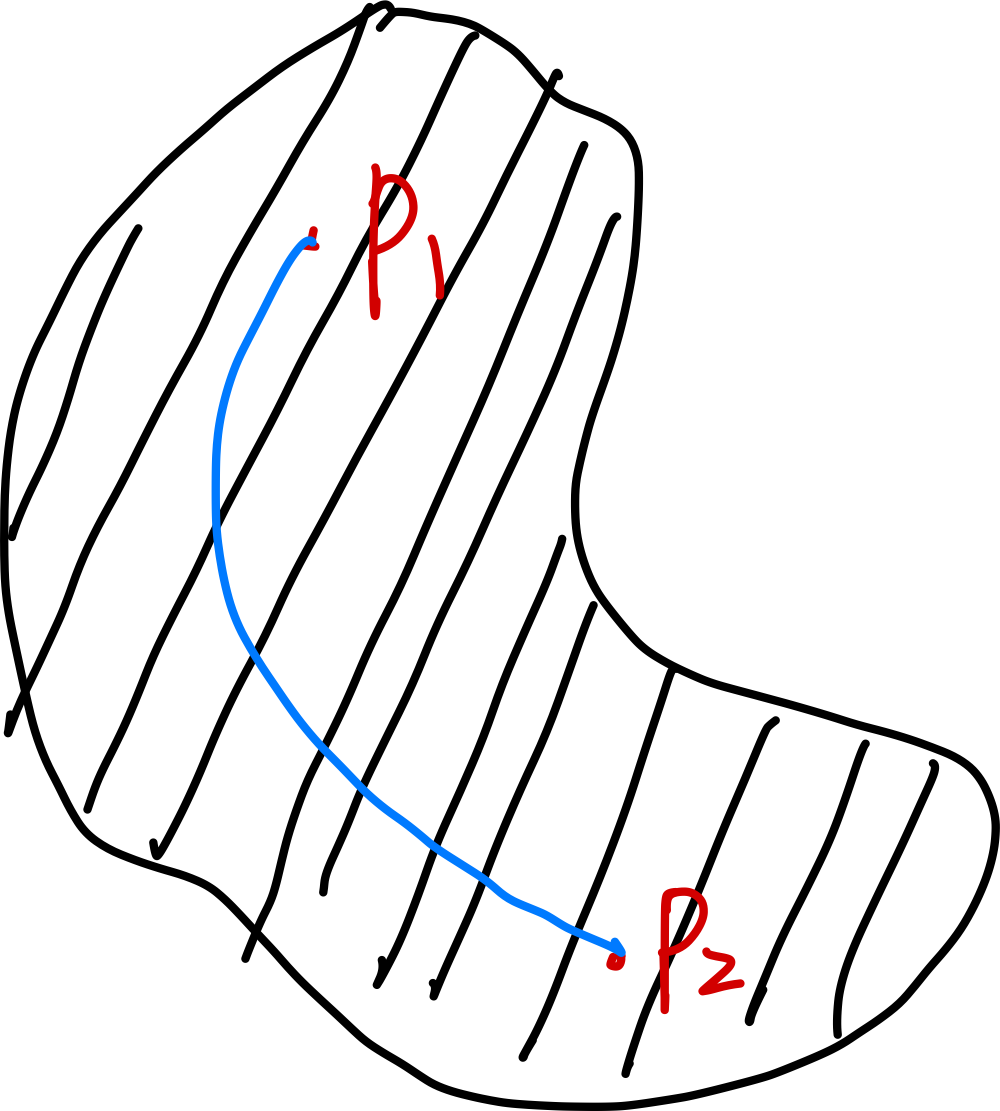
\includegraphics[scale=0.2]{"Chapter 03 images/pic1.png"}
        % \caption{}
        \label{pic1}
    \end{wrapfigure}

    元位移\(\rmd \overrightarrow{r}\)、元路程\(\rmd s\)

    则元功\(\rmd W = \overrightarrow{F} \cdot \rmd \overrightarrow{r} =
    F \cos \alpha \rmd s\)

    积分:

    \begin{align}
        W=\int_A^B \overrightarrow{F} \cdot \rmd \overrightarrow{r}=\int_A^B F \cos \alpha \mathrm{~d} s
    \end{align}

    \begin{enumerate}
        \item 功的正负
            $$
                \begin{cases}0^{\circ}<\alpha<90^{\circ}, & \mathrm{d} W>0 \\
                90^{\circ}<\alpha<180^{\circ}, & \mathrm{d} W<0 \\
                \alpha=90^{\circ}, \text{即} \overrightarrow{F} \perp \rmd \overrightarrow{r}, & \rmd W=0\end{cases}
            $$
        \item 做功的图示\\
            {
            \centering
            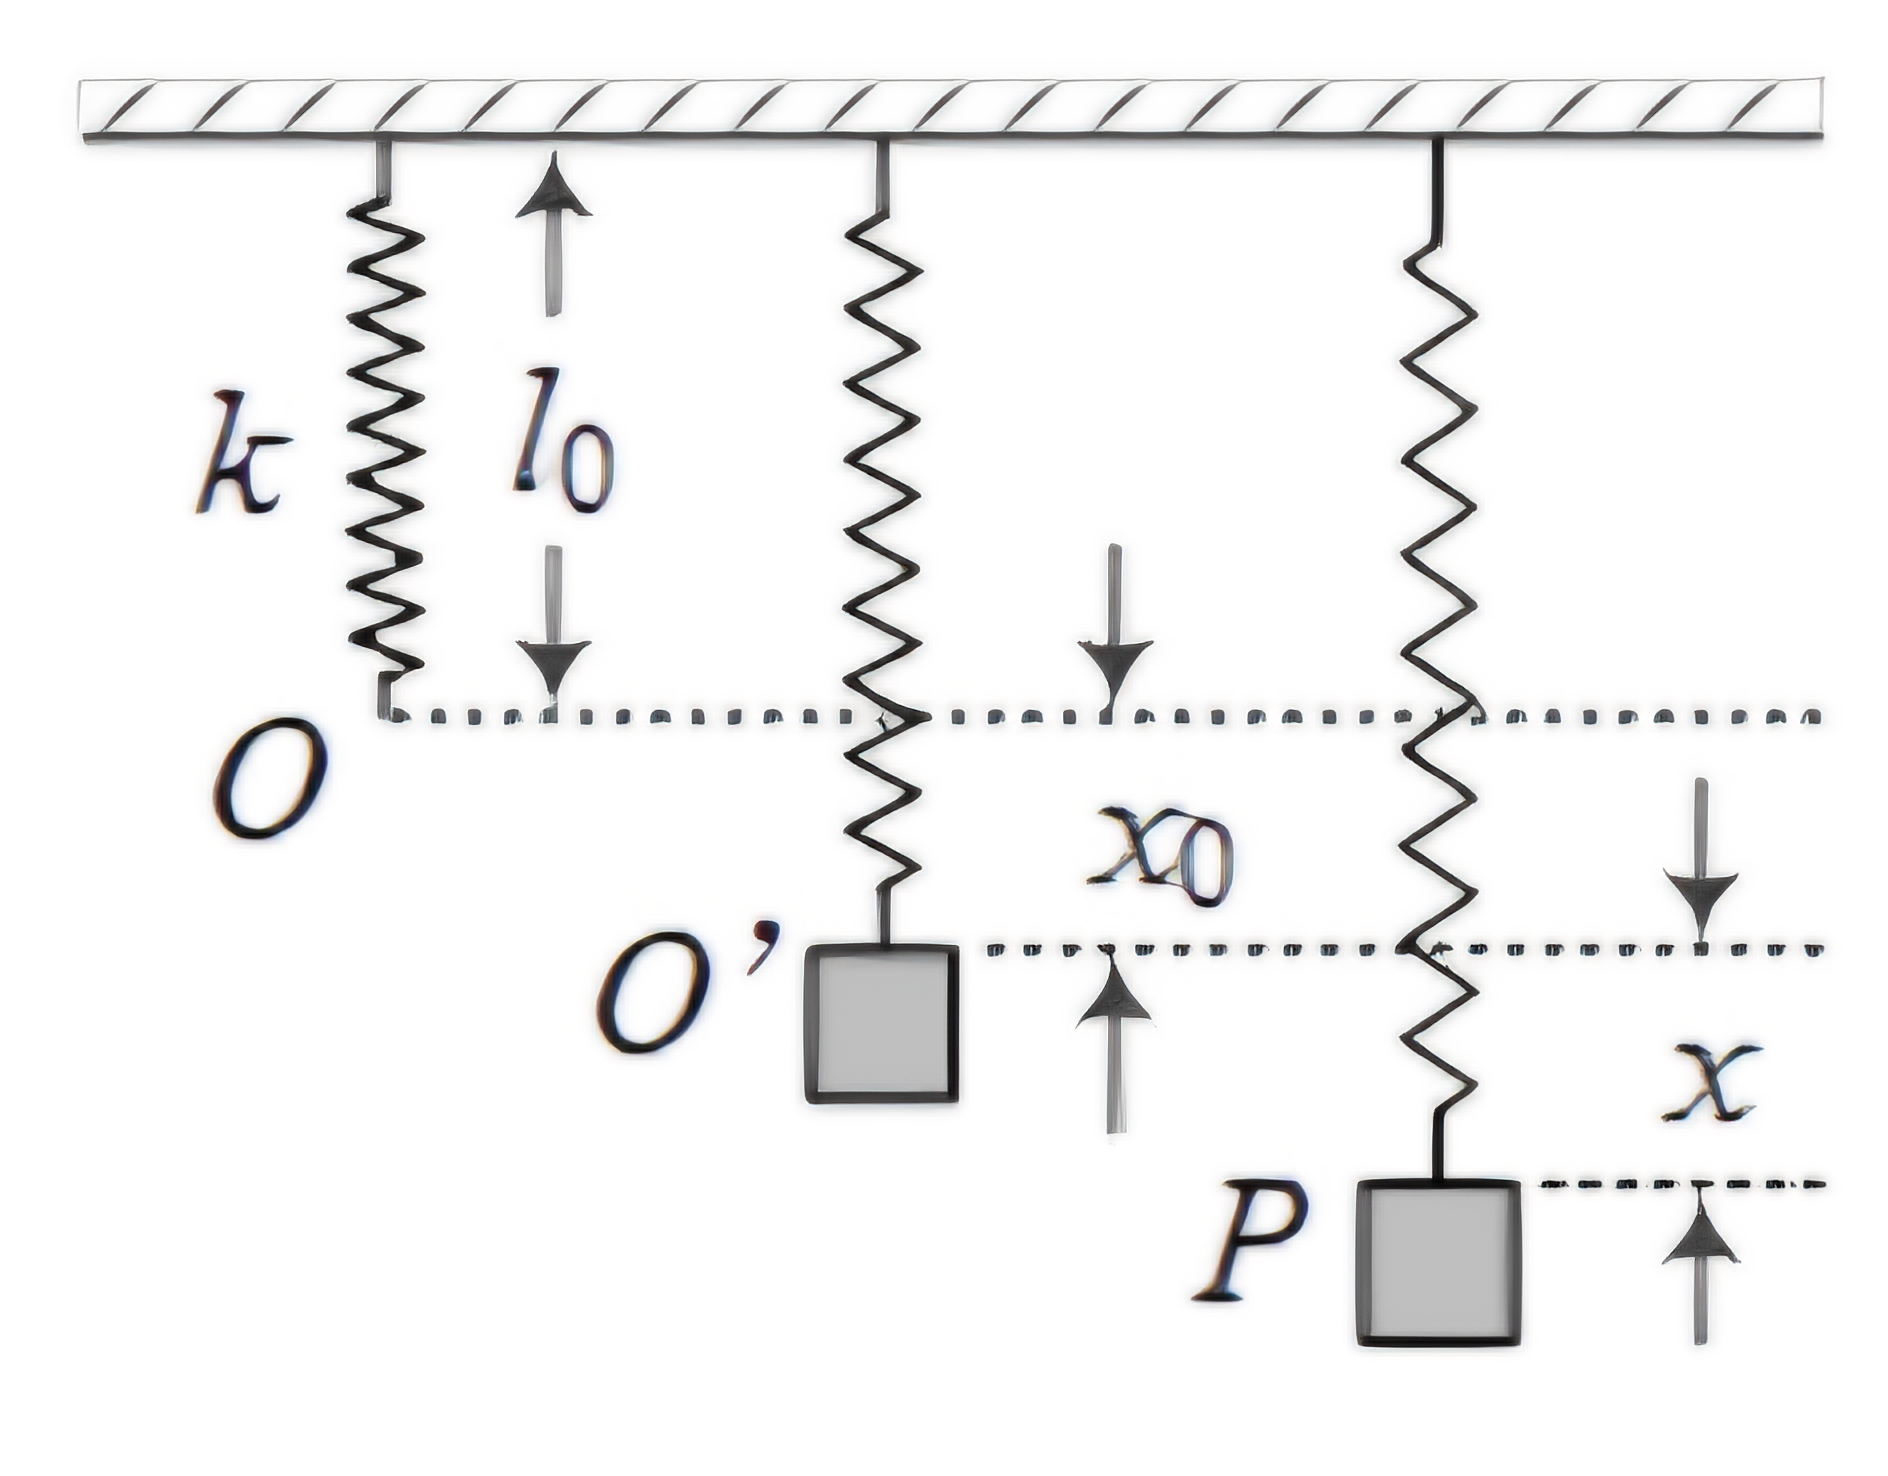
\includegraphics[scale=0.2]{"Chapter 03 images/pic2.png"}
            }
        \item 功是一个过程量,与路径有关。
        \item 合力的功,等于各分力的功的\textbf{代数和}
            \begin{align*}
                \overrightarrow{F}=F_x \overrightarrow{i}+F_y \overrightarrow{j}+F_z \overrightarrow{k} \\
                \mathrm{~d} \overrightarrow{r}=\mathrm{d} x \overrightarrow{i}+\mathrm{d} y \overrightarrow{j}+\mathrm{d} z \overrightarrow{k}
            \end{align*}
            则
            \begin{align*}
                W=\int_A^B \overrightarrow{F} \cdot \mathrm{~d} \overrightarrow{r}=
                \int_A^B\left(F_x \mathrm{~d} x+F_y \mathrm{~d} y+F_z \mathrm{~d} z\right)
            \end{align*}
            又有$W_x=\int_{x_1}^{x_B} F_x \mathrm{~d} x$、$W_y=\int_{y_1}^{y_B} F_y \mathrm{~d} y$、
            $W_z=\int_{z_1}^{z_B} F_z\mathrm{~d} z$。\\
            于是
            \[
                W = W_x + W_y + W_z
            \]

    \end{enumerate}
    
\subsection{功率}

    \textbf{平均功率}$\overline{P}=\frac{\Delta W}{\Delta t}$

    \textbf{瞬时功率}
    
    \begin{align}
        P=\lim _{\Delta t \rightarrow 0} \frac{\Delta W}{\Delta t}=\frac{\mathrm{d} W}{\mathrm{~d} t}=\overrightarrow{F} \cdot \overrightarrow{v}
    \end{align}

    即

    \begin{align}
        P = Fv\cos\alpha
    \end{align}
    
\subsection{动能定理}

\subsubsection{质点的动能定理}

    \begin{wrapfigure}{r}{4cm}
        \centering
        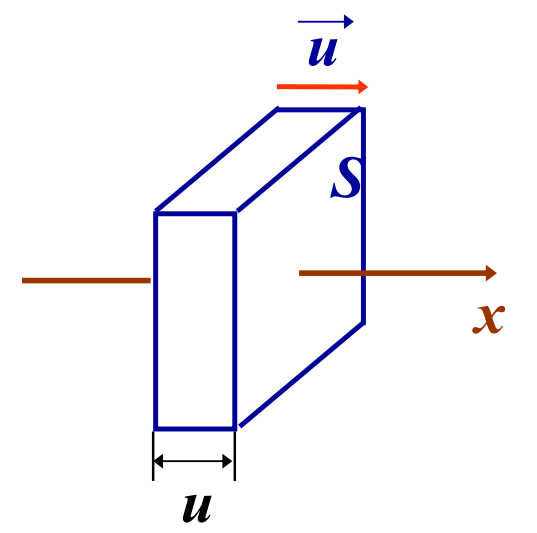
\includegraphics[scale=0.2]{"Chapter 03 images/pic3.png"}
        % \caption{}
        \label{pic3}
    \end{wrapfigure}

    $$
    \begin{aligned}
        W & =\int \overrightarrow{F} \cdot \mathrm{~d} \overrightarrow{r} \\
        & =\int F_{\mathrm{t}}|\mathrm{~d} \overrightarrow{r}|=\int F_{\mathrm{t}} \mathrm{~d} s
    \end{aligned}
    $$

    而

    $$
        F_{\mathrm{t}}=m \frac{\mathrm{~d} v}{\mathrm{~d} t}
    $$

    于是

    $$
        \begin{aligned}
        W & =\int_{v_1}^{v_2} m v \mathrm{~d} v \\
        & =\frac{1}{2} m v_2^2-\frac{1}{2} m v_1^2
        \end{aligned}
    $$

    即

    \begin{equation}
        W=\frac{1}{2} m v_2^2-\frac{1}{2} m v_1^2=E_{\mathrm{k} 2}-E_{\mathrm{k} 1}
    \end{equation}

    合外力对质点所作的功,等于质点动能的增量。——质点的动能定理

    \begin{enumerate}
        \item 功是\textbf{过程量},动能是\textbf{状态量};
        \item 功和动能依赖于惯性系的选取,但对不同惯性系动能定理形式相同。
    \end{enumerate}

\subsubsection{质点系的动能定理}

    \textbf{质点系}:由有限个或无限个质点组成的系统。(可以是固体也可以是液体,它概括了力学中最普遍的研究对象)

    \textbf{内力和外力}:质点系以外的物体作用于质点系内各质点的力称为外力,
    质点系内各质点之问的相互作用力称为内力,外力和内力的区分完全洪定于质点系(研究对象)的选取。

    \textbf{质点系内力的功}:一切内力矢量和恒等于零。但一般情烷下,所有内力作功的总和并不为零。
    例如,两个彼此相互吸引的物体,移动一段位移,都作正功。

    \textbf{质点系的动能定理}

    由质点动能定理$W=E_{k 2}-E_{k 1}=\Delta E_k$

    得

    \begin{equation}
        W_e+W_i=\sum_i\left(\frac{1}{2} m_i v_{i 2}^2-\frac{1}{2} m_i v_{i 1}^2\right)=E_{k 2}-E_{k 1}=\Delta E_k
    \end{equation}

    意义:合外力所做的功等于系统动能的增量。

\section{保守力、势能、成对力的功}

\subsection{保守力}

\subsubsection{万有引力}

    \begin{wrapfigure}{r}{4cm}
        \centering
        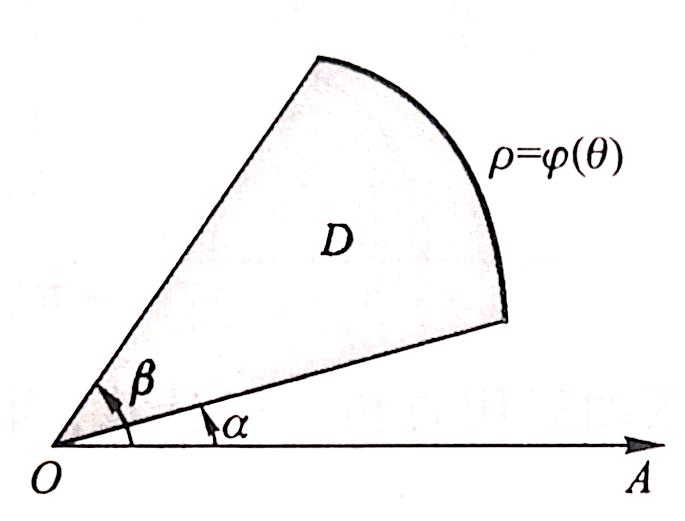
\includegraphics[scale=0.2]{"Chapter 03 images/pic4.png"}
        % \caption{}
        \label{pic4}
    \end{wrapfigure}

    \(m_{E}\)对\(m\)的万有引力为

    $$
        \overrightarrow{F}=-G \frac{m_{E} m}{r^2} \overrightarrow{e}_r
    $$

    \(m\)移动\(\rmd \overrightarrow{r}\)时,\(\overrightarrow{F}\)做元功为

    $$
        \rmd W = \overrightarrow{F} \cdot \rmd \overrightarrow{r}
        =-G \frac{m_{E} m}{r^2} \overrightarrow{e}_r \cdot \rmd \overrightarrow{r}
    $$

    \(m\)从\(A\)到\(B\)时,\(\overrightarrow{F}\)做功为

    $$
    W=\int \overrightarrow{F} \cdot \rmd \overrightarrow{r}
    =\int_A^B-G \frac{m_{E} m}{r^2} \overrightarrow{e}_r \cdot \rmd \overrightarrow{r}
    $$

    \begin{wrapfigure}{r}{4cm}
        \centering
        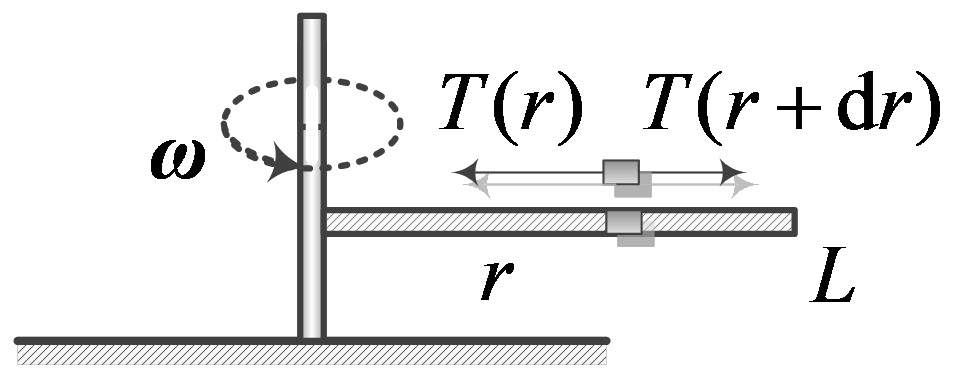
\includegraphics[scale=0.15]{"Chapter 03 images/pic6.png"}
        % \caption{}
        \label{pic6}
    \end{wrapfigure}

    其中,$\overrightarrow{e}_r \cdot \mathrm{~d} \overrightarrow{r}=
    \left|\overrightarrow{e}_r\right| \cdot|\mathrm{d} \overrightarrow{r}| \cos \alpha=\mathrm{d} r$

    即

    $$
        W=\int_{r_A}^{r_B} \left(-G \frac{m_E m}{r^2}\right) \rmd r
    $$

    于是

    \begin{equation}
        W=G m_{E} m\left(\frac{1}{r_B}-\frac{1}{r_A}\right)
    \end{equation}

    \textbf{做功特点}:做功大小只与物体的始末位置有关,与路径无关。

\subsubsection{弹性力做功}

    \begin{wrapfigure}{r}{4cm}
        \centering
        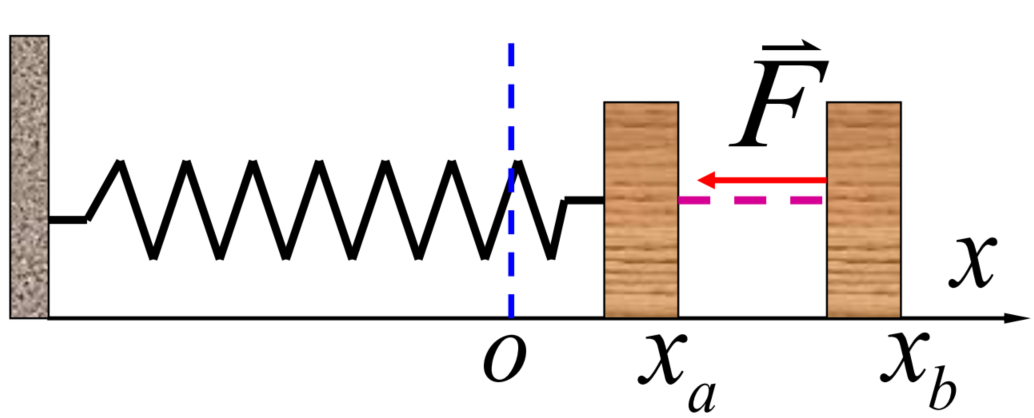
\includegraphics[scale=0.12]{"Chapter 03 images/pic5.png"}
        % \caption{}
        \label{pic5}
    \end{wrapfigure}

    弹性力\(\overrightarrow{F} = -kx\overrightarrow{i}\),则元功

    \[
        \rmd W = -kx \rmd x
    \]

    于是

    \begin{equation}
        W=\int_{x_a}^{x_b} F \mathrm{~d} x=\int_{x_a}^{x_b}-k x \mathrm{~d} x=-\left(\frac{1}{2} k x_b^2-\frac{1}{2} k x_a^2\right)
    \end{equation}

    \textbf{做功特点}:做功大小只与物体的始末位置有关,与路径无关。

\subsubsection{保守力与非保守力的定义}

    \textbf{保守力}:作功与路径无关,仅决定于始、末位置的力。

    质点沿任意闭合路径运动一周时,保守力对它作功为零。

    \textbf{非保守力}:所作的功与路径有关的力。(如摩擦力)

\subsection{势能}

\subsubsection{定义}

    因相对位置而具有的作功本领称为势能或位能(因有速度而具有的作功本领称为动能)。
    势能与质点的位置有关。

    如引力势能

    \[
        E_{\mathrm{p}} = -G \frac{m_{E}m}{r}
    \]

    如弹性势能

    \[
        E_{\mathrm{p}} = \frac{1}{2}kx^2
    \]

\subsubsection{保守力做功}

    \textbf{保守力做的功等于势能的减少},即

    \begin{equation}
        W =-\left(E_{\mathrm{p} 2}-E_{\mathrm{p} 1}\right)=-\Delta E_{\mathrm{p}}
    \end{equation}

\subsubsection{保守力做功势能的计算}

    令\(E_{\mathrm{p0}} = 0\),则

    \begin{equation}
        E_{\mathrm{p}}(x, y, z)=\int_{(x, y, z)}^{E_{\mathrm{p} 0}=0} \overrightarrow{F} \cdot \mathrm{~d} \overrightarrow{r}
    \end{equation}

    \begin{enumerate}
        \item 势能是\textbf{状态的函数},$E_{\mathrm{p}}=E_{\mathrm{p}}(x, y, z)$;
        \item 势能具有\textbf{相对性},势能大小与势能零点的选取有关;
        \item 势能是\textbf{属于系统}的;
        \item \textbf{势能差}与势能零点的选取无关。
    \end{enumerate}

\subsubsection{势能曲线}

    \begin{figure}[htbp]
        \centering
        \subfigure
        {
            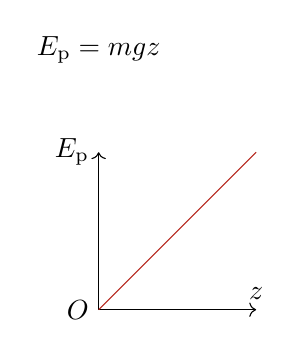
\begin{tikzpicture}
                \coordinate[label=left:$E_{\mathrm{p}}$] (E_p) at (0,2);
                \coordinate[label=above:$z$] (z) at (2,0);
                \coordinate[label=left:$O$] (O) at (0,0);
                \coordinate[label={above:$E_{\mathrm{p}} = mg z$}] (formula) at (0,3);
                \draw[->] (O) -- (z);
                \draw[->] (O) -- (E_p);
                \draw[domain=0:2,BrickRed] plot(\x,{\x});
            \end{tikzpicture}
        }
        \subfigure
        {
            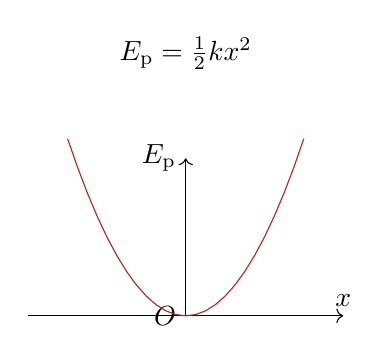
\begin{tikzpicture}
                \coordinate[label=left:$E_{\mathrm{p}}$] (E_p) at (0,2);
                \coordinate[label=above:$x$] (x) at (2,0);
                \coordinate[label=left:$O$] (O) at (0,0);
                \coordinate[label={above:$E_{\mathrm{p}} = \frac{1}{2}kx^2$}] (formula) at (0,3);
                \draw[->] (-2,0) -- (x);
                \draw[->] (O) -- (E_p);
                \draw[domain=-1.5:1.5,BrickRed] plot(\x,{\x*\x});
            \end{tikzpicture}
        }
        \subfigure
        {
            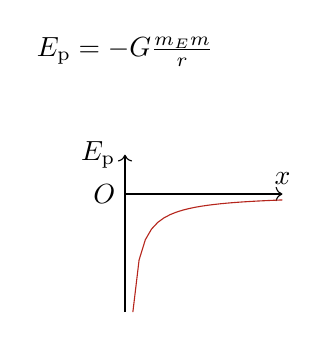
\begin{tikzpicture}
                \coordinate[label=left:$E_{\mathrm{p}}$] (E_p) at (0,0.5);
                \coordinate[label=above:$x$] (x) at (2,0);
                \coordinate[label=left:$O$] (O) at (0,0);
                \coordinate[label={above:$E_{\mathrm{p}} = -G \frac{m_{E}m}{r}$}] (formula) at (0,1.5);
                \draw[->] (O) -- (x);
                \draw[->] (0,-1.5) -- (E_p);
                \draw[domain=0.1:2,BrickRed] plot(\x,{-0.15/\x});
            \end{tikzpicture}
        }
        % \caption{}
    \end{figure}

    把势能和相对位置的关系绘成曲线,便得到势能曲线。
            
    通过势能曲线,可以显示出系统总机械能,动能和势能间的关系
    $E=E_k+E_p$,由 $E_{\mathrm{k}} \geq 0$ ,可以根据曲线的形状讨论物体的运动。

\subsubsection{由势能求表达式}

    可以根据势能\(E_{\mathrm{p}}\left(x,y,z\right)\)的情况,判断物体在各个位置所受保守力的大小和方向:

    $$
        \rmd W=F_x \rmd x=-\rmd E_p
    $$

    则

    \begin{equation}
        F_x=-\frac{\rmd E_p}{\rmd x}
    \end{equation}

    如果势能是位置\(\left(x,y,z\right)\)的多元函数,则

    \begin{equation}
        \overrightarrow{F}=F_x \overrightarrow{i}+F_y \overrightarrow{j}+F_z \overrightarrow{k}=
        -\left(\frac{\partial E_p}{\partial x} \overrightarrow{i}+\frac{\partial E_p}{\partial y} \overrightarrow{j}+\frac{\partial E_p}{\partial z} \overrightarrow{k}\right)
    \end{equation}

\subsection{成对的力的功}

    力总是成对的,无论是保守力还是非保守力。
    
    设质量为$m_1$和$m_2$的两个物体分别受到 $F_1$ 和 $F_2$ 的力,
    且 $\overrightarrow{F}_1=-\overrightarrow{F}_2$在$\rmd t$时间内位移为 $\rmd r_1$
    和 $\rmd r_2$ ,质点 2 相对于质点 1 的相对位移 $\rmd \overrightarrow{r}^{\prime}$有
    $\rmd \overrightarrow{r}_2=d \overrightarrow{r}_1+\rmd r^{\prime}$ 则元功为:
    
    $$
        \begin{aligned}
        & \rmd W_1=\overrightarrow{F}_1 \cdot \rmd \overrightarrow{r}_1 \\
        & \rmd W_2=\overrightarrow{F}_2 \cdot \rmd \overrightarrow{r}_2
        \end{aligned}
    $$

    这一对力所作元功之和为:

    $$
    \begin{aligned}
        & \rmd W=\overrightarrow{F}_1 \cdot \rmd \overrightarrow{r}_1+\overrightarrow{F}_2 \cdot \rmd \overrightarrow{r}_2=\overrightarrow{F}_1 \cdot\rmd\overrightarrow{r}_1+\overrightarrow{F}_2 \cdot\left(d \overrightarrow{r}_1+d \overrightarrow{r}^{\prime}\right) \\
        & =\left(-\overrightarrow{F}_2+\overrightarrow{F}_2\right) \cdot\rmd\overrightarrow{r}_1+\overrightarrow{F}_2 \cdot\rmd\overrightarrow{r}^{\prime} \quad \\
        & =\overrightarrow{F}_2 \cdot\rmd\overrightarrow{r}^{\prime}
    \end{aligned}
    $$

    \begin{enumerate}
        \item 成对力的功只与作用力和相对位移有关;
        \item 成对力的总功具有与参考系选择无关的不变性质。\\
            为方便起见,计算时常认为其中一个质点静止,并以该质点所在位置为原点,
            再计算另一质点受力所做的功,这就是一对力的功。
        \item 在无相对位移或相对位移与一对力垂直的情况下,一对力的功必为零。
    \end{enumerate}

\section{功能原理、机械能守恒定律}

\subsection{质点系功能原理}

    \textbf{系统的机械能}:动能与势能的综合称为机械能,即

    \[
        E = E_{\mathrm{k}} + E_{\mathrm{p}}
    \]

    \textbf{内力的功可分为}:保守内力的功和非保守内力功

    \[
        W^{\mathrm{in}} = \sum_{i} W_{i}^{\mathrm{in}} =
        W_{\mathrm{c}}^{\mathrm{in}} + W_{\mathrm{nc}}^{\mathrm{in}}
    \]

    由势能的定义,保守内力的功总等于系统势能的减少:

    \[
        W_{\mathrm{c}}^{\mathrm{in}} = - \Delta E_{\mathrm{p}}
    \]

    \textbf{系统的功能原理}

    (由质点系的动能定理)

    \[
        W^{\mathrm{ex}} + W^{\mathrm{in}} = W^{\mathrm{ex}} + W_{\mathrm{c}}^{\mathrm{in}}
        + W_{\mathrm{nc}}^{\mathrm{in}} = W^{\mathrm{ex}} - \Delta E_{\mathrm{p}} +
        W_{\mathrm{nc}}^{\mathrm{in}} = \Delta E_{\mathrm{k}}
    \]

    于是,

    \begin{align}
        \Delta E = \Delta E_{\mathrm{k}} + \Delta E_{\mathrm{p}} =
        W^{\mathrm{ex}} + W_{\mathrm{nc}}^{\mathrm{in}}
    \end{align}

    在选定的质点系内,在任一过程中,质点系总机械能的增量等于\textbf{所有外力}的功与\textbf{非保守内力}的功的代数和。

    非保守内力的功将导致机械能与其他形式的能量转换。

\subsection{机械能守恒定律}

    由功能原理:$\Delta E = \Delta E_{\mathrm{k}} + \Delta E_{\mathrm{p}} =
    W^{\mathrm{ex}} + W_{\mathrm{nc}}^{\mathrm{in}}$。

    如果$W^{\mathrm{ex}} + W_{\mathrm{nc}}^{\mathrm{in}} = 0$,则

    \[
        \Delta E = \Delta E_{\mathrm{k}} + \Delta E_{\mathrm{p}} = 0
    \]

    即,如是系统内只有保守内力做功,其他内力和一切外力都不做功,或元功之和为零,
    则系统内各物体的动能和势能可以相互转换,但总机械能保持不变。

    \begin{enumerate}
        \item 质点系的机械能守恒的条件是:在一个过程中,既没有外力做功,也没有非保守内力(如摩擦力、爆炸力、流体的黏性阻力等耗散力)做功,或者外力和非保守内力做的总功为零。
        \item 在满足守恒条件时,质点系的总机械能可以在动能和系统势能之间转化,也可以在系统内各物体之问转移,但在转化和转移过程中保特总机械能不变。
    \end{enumerate}

\subsection{能量守恒定律}

    对于一个不受外界影响的封闭系统(有时也称为孤立系统),系统内各种不同形式的能量可以互相转化,也可以从系统的一部分转移到另一部分,
    但不论系统内发生什么过程,能量既不会消失也不会产生,系统的总能量恒定不变。这就是能量守恒定律 (law of conservation of energy)。

\subsection{动量与能量的比较}

    \begin{table}[htbp]
        \centering
        \begin{tabular}{|l|ll|}
            \hline
            \textbf{物理量} & \multicolumn{1}{l|}{\textbf{动量(momentum)}}                    & \textbf{能量(kinetic energy)}      \\ \hline
            表达式          & \multicolumn{1}{l|}{\(\overrightarrow{p} = m\overrightarrow{v}\)} & \(E_{\mathrm{k}} = \frac{1}{2}mv^2\) \\ \hline
            单位  & \multicolumn{1}{l|}{\(\mathrm{kg \cdot m / s}\)} & \(\mathrm{J}\)                  \\ \hline
            性质  & \multicolumn{1}{l|}{矢量}                      & 标量                          \\ \hline
            关系  & \multicolumn{2}{c|}{\(\dfrac{p^2}{2m} = E_{\mathrm{k}}\)}                       \\ \hline
            变化量 & \multicolumn{1}{l|}{\(\Delta p\)由力的冲量决定}         & \(\Delta E_{\mathrm{k}}\)由力的功决定 \\ \hline
        \end{tabular}
    \end{table}

    另外,\(\Delta p\)与惯性系的选择无关,\(\Delta E_{\mathrm{k}}\)随惯性系的不同而不同。

\section{碰撞、碰撞定律、质心运动定律}

\subsection{碰撞}

    \textbf{定义}

    两个或两个以上的物体相遇,相遇时物体之间的相互作用,仅持续极为短暂的时间。

    \textbf{特点}

    \begin{enumerate}
        \item 作用时间极短;
        \item 作用力变化极快;
        \item 作用力峰值极大;
        \item 过程中物体发生形变;
        \item 可认为碰撞过程中只受内力(\(\overrightarrow{F}^{\mathrm{ex}} \ll \overrightarrow{F}^{\mathrm{in}}\)),故遵守动量守恒定律(\(\sum_{i} \overrightarrow{p}_{i} = \overrightarrow{C}\))。
    \end{enumerate}

\subsection{碰撞定律}

    \begin{align}
        e = \frac{v_2 - v_1}{v_{10} - v_{20}}
    \end{align}

    即

    $$
    e = \frac{\text{分离速度}}{\text{接近速度}}
    $$

    (\(e\)称恢复系数,由材料性质决定。)

\subsection{碰撞的分类}

\subsubsection{完全弹性碰撞}

    恢复系数\(e=1\),\(v_2-v_1=v_{10} - v_{20}\)。
    
    碰撞后形变能完全恢复,没有机械能的损失,系统碰撞前后机械能守恒。

    动量守恒,机械能守恒。

    对于\textbf{完全弹性对心碰撞}:

    $$
        \left\{\begin{array}{l}
        m_1 v_{10}+m_2 v_{20}=m_1 v_1+m_2 v_2 \\
        \dfrac{1}{2} m_1 v_{10}^2+\dfrac{1}{2} m_2 v_{20}^2=\dfrac{1}{2} m_1 v_1^3+\dfrac{1}{2} m_2 v_2^2
        \end{array}\right.
    $$

    联立方程解得

    \begin{align}
        \left\{\begin{array}{l}
            v_1=\dfrac{m_1-m_2}{m_1+m_2} v_{10}+\dfrac{2 m_2}{m_1+m_2} v_{20} \\
            v_2=\dfrac{2 m_1}{m_1+m_2} v_{10}+\dfrac{m_2-m_1}{m_1+m_2} v_{20}
        \end{array}\right.
    \end{align}

\subsubsection{完全非弹性碰撞}

    恢复系数\(e=0\),\(v_2=v_1=v\)。
    
    碰撞后二者没有分开,并以共同的速度一起运动。物体碰撞后已经完全不可能恢复形变。

    动量守恒,机械能不守恒。

    对于\textbf{完全非弹性对心碰撞}:

    由

    $$
        m_1 v_{10}+m_2 v_{20}=\left(m_1+m_2\right) v
    $$

    解得

    \begin{equation}
        v=\frac{m_1 v_{10}+m_2 v_{20}}{m_1+m_2}
    \end{equation}

    损失能量

    \begin{equation}
        \Delta E=\frac{1}{2} m_1 v_{10}^2+\frac{1}{2} m_2 v_{20}^2-\frac{1}{2}\left(m_1+m_2\right) v^2
    \end{equation}

\subsubsection{非完全弹性碰撞}

    恢复系数\(0<e<1\),\(v_2=v_1=e\left(v_{10} - v_{20}\right)\)。

    碰撞后形变不能完全恢复,一部分机械能将被转变为其他形式的能量(如热能)。

    动量守恒,机械能不守恒。

\subsubsection{斜碰撞}

    碰撞前与碰撞后的速度不在一条直线上。

    例如,一光滑球与另外静止的光滑球相碰。如果两者均为弹性球,且碰后两者的运动方向垂直,
    则两小球质量必然相等

\subsection{质心}

\subsubsection{定义}

    在研究质点系统问题中,与质点系统质量分布有关的一个代表点,它的位置在平均意义上代表
    着质量分布中心。

\subsubsection{质心位置}

    \begin{align}
        \overrightarrow{r}_{\mathrm{C}} = \frac{\sum_{i} m_ir_i}{M}
    \end{align}

    即

    $$
        \left\{\begin{array}{l}
        x_C=\frac{\sum m_i x_i}{M} \\
        y_C=\frac{\sum m_i y_i}{M} \\
        z_C=\frac{\sum m_i z_i}{M}
        \end{array}\right.
    $$

    则质量连续分布的系统的质心位置

    $$
        \overrightarrow{r}_C=\int \overrightarrow{r} \rmd m / M
    $$

    即

    $$
        \left\{\begin{array}{l}
            x_c=\frac{\int x \mathrm{~d} m}{M} \\
            y_c=\frac{\int y \mathrm{~d} m}{M} \\
            z_c=\frac{\int z \mathrm{~d} m}{M}
        \end{array}\right.
    $$

    \textbf{注意}

    \begin{enumerate}
        \item 质心不同于重心,物体体积不太大时,两者重和;物体远离地球时不受重力,"重心"失去意义,"质心"仍在。
        \item 当外力的作用线通过质心时,物体只作平动,没有转动,就好像物体的质量都集中在质心这一点上。
    \end{enumerate}

\subsubsection{质心速度}

    \begin{equation}
        \overrightarrow{v}_C=\frac{\rmd \overrightarrow{r}_C}{\rmd t}=\frac{\sum m_i \frac{\rmd \overrightarrow{r}_i}{\rmd t}}{M}=\frac{\sum m_i \overrightarrow{v}_i}{M}
    \end{equation}

\subsubsection{质心加速度}

    \begin{equation}
        \overrightarrow{v}_C=\frac{\rmd \overrightarrow{r}_C}{\rmd t}=\frac{\sum m_i \frac{\rmd \overrightarrow{r}_i}{\rmd t}}{M}=\frac{\sum m_i \overrightarrow{v}_i}{M}
    \end{equation}

\subsection{质心运动定律}

    质心的加速度与质点系所受外力的矢量和成正比,与质点系的总质量成反比,质心的加速度与内力无关。

    \begin{equation}
        \overrightarrow{a}_C=\frac{\sum \overrightarrow{F}_i}{\sum m_i}=\frac{\sum \overrightarrow{F}_i}{M}
    \end{equation}


\section{例题}

\subsection{Problem 1}

    \begin{wrapfigure}{r}{4cm}
        \centering
        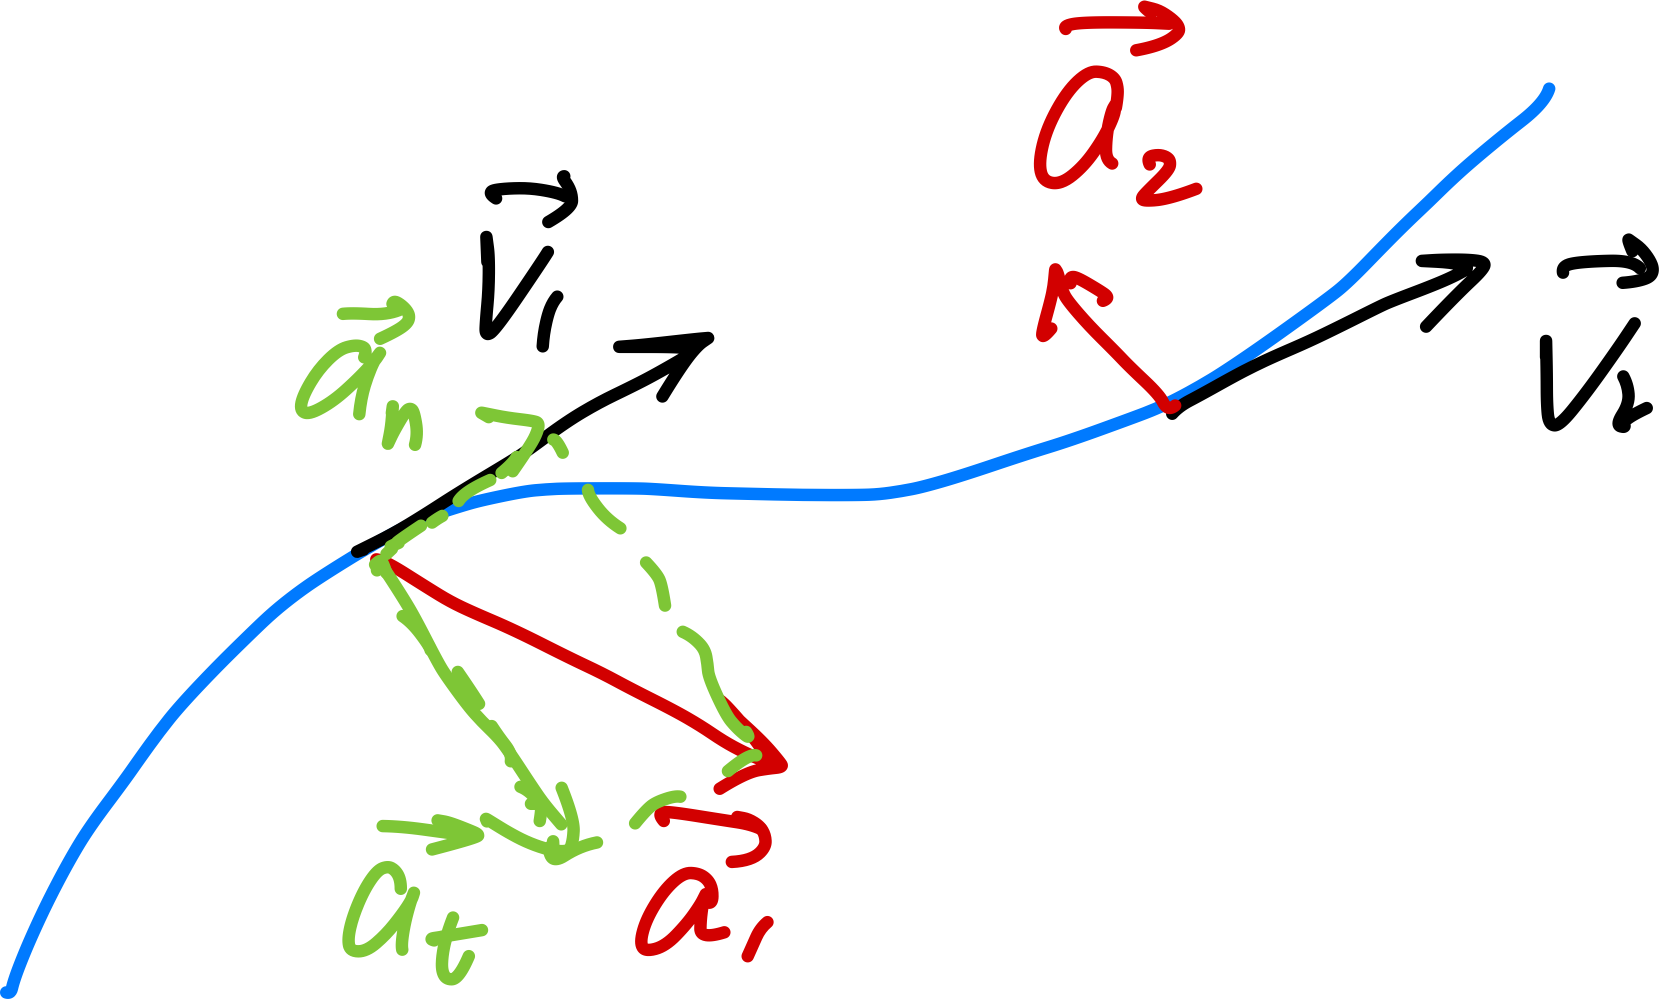
\includegraphics[scale=0.12]{"Chapter 03 images/pic7.png"}
        % \caption{}
        \label{pic7}
    \end{wrapfigure}

    在宇宙中有密度为\(\rho\)的尘埃,这些尘埃相对惯性参考系是静止的。有一质量为\(m_0\)的宇宙飞船以初速度\(v_0\)
    穿过宇宙尘埃,由于尘埃粘贴到飞船上,致使飞船的速度发生改变。求飞船的速度与其在尘埃中飞行时间的关系。
    (设想飞船的外形是截面积为\(S\)的圆柱体)
    \vspace{1em}

    \textbf{Solution}
    \vspace{1em}

    尘埃与飞船作完全非弹性碰撞,把它们作为一个系统,则动量守恒:

    $$
        m_0 v_0+\left(m-m_0\right) \times 0=m v
    $$

    解得

    \[
        m = \frac{m_0v_0}{v}
    \]

    所有与飞船迎面相撞的尘埃都会粘贴到飞船上。考查\(\rmd t\)时间内与飞船迎面相撞的尘埃:

    \[
        \rmd m = \rho Sv\rmd t
    \]

    又因为

    \[
        m = \frac{m_0v_0}{v}
    \]

    所以

    \[
        \rmd m = -\frac{m_0v_0}{v^2} \rmd v = \rho Sv\rmd t
    \]

    由

    $$
        -\int_{v_0}^v \frac{d v}{v^3}=\frac{\rho S}{m_0 v_0} \int_0^t d t
    $$

    得

    $$
        v=v_0\sqrt{\frac{m_0}{2 \rho S v_0 t+m_0}}
    $$

\subsection{Problem 2}

    \begin{wrapfigure}{r}{4cm}
        \centering
        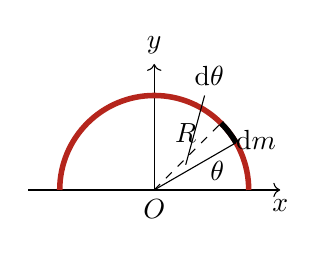
\begin{tikzpicture}[scale=0.8]
            \coordinate[label=below:$x$] (x) at (2,0);
            \coordinate[label=above:$y$] (y) at (0,2);
            \coordinate[label=below:$O$] (O) at (0,0);
            \draw[->] (O) -- (y);
            \draw[->] (-2,0) -- (x);
            \draw[BrickRed, line width=2pt] (1.5,0) arc (0:180:1.5);
            \draw[Black, line width=2pt] (0.75*1.732,0.75) arc (30:45:1.5);
            \draw[dashed] (O) -- (0.75*1.414,0.75*1.414);
            \draw (O) -- (0.75*1.732,0.75);
            \coordinate[label=above:$\theta$] (theta) at (1,0);
            \coordinate[label=above:$R$] (R) at (0.5,0.6);
            \coordinate[label=above:$\rmd \theta$] (dtheta) at (0.8,1.5);
            \draw (0.5,0.4) -- (dtheta);
            \coordinate[label=right:$\rmd m$] (dm) at (1,0.8);
        \end{tikzpicture}
    \end{wrapfigure}

    已知一圆环半径为\(R\),质量为\(M\),求它的质心位置。
    \vspace{1em}

    \textbf{Solution}
    \vspace{1em}

    建坐标系如图,取一小段长度\(\rmd l\)则其质量为\(\rmd m = \lambda \rmd l\)。

    又\(\rmd l = R \rmd \theta\),故\(\rmd m = \frac{M}{\uppi R} R \rmd \theta\)

    而\(x = R\cos \theta\),\(y = R\sin \theta\)

    故

    $$
        y_c=\frac{\int y \mathrm{~d} m}{M}=\frac{\int_0^\pi R \sin \theta \frac{M}{\pi R} R \mathrm{~d} \theta}{M}=\frac{2 R}{\pi}
    $$

    由对称性可知,

    $$
        x_c = 0
    $$

\end{document}
